\section{ALLOY}
\subsection{Model}
\begin{figure}[H]
	\centering
	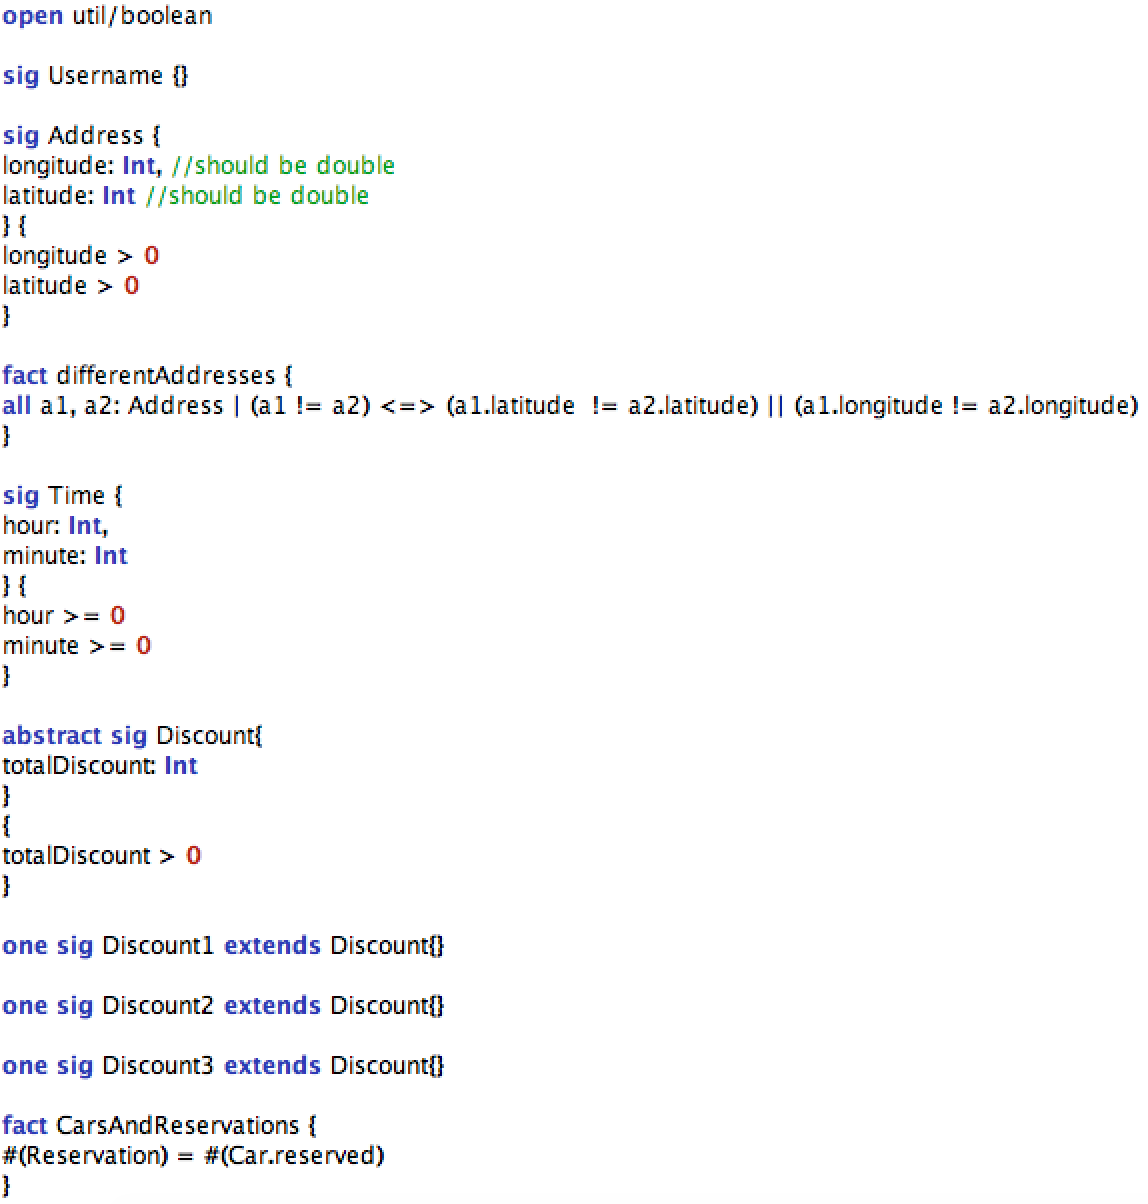
\includegraphics[width=14cm]{AlloyModel1}
\end{figure}
\begin{figure}[H]
	\centering
	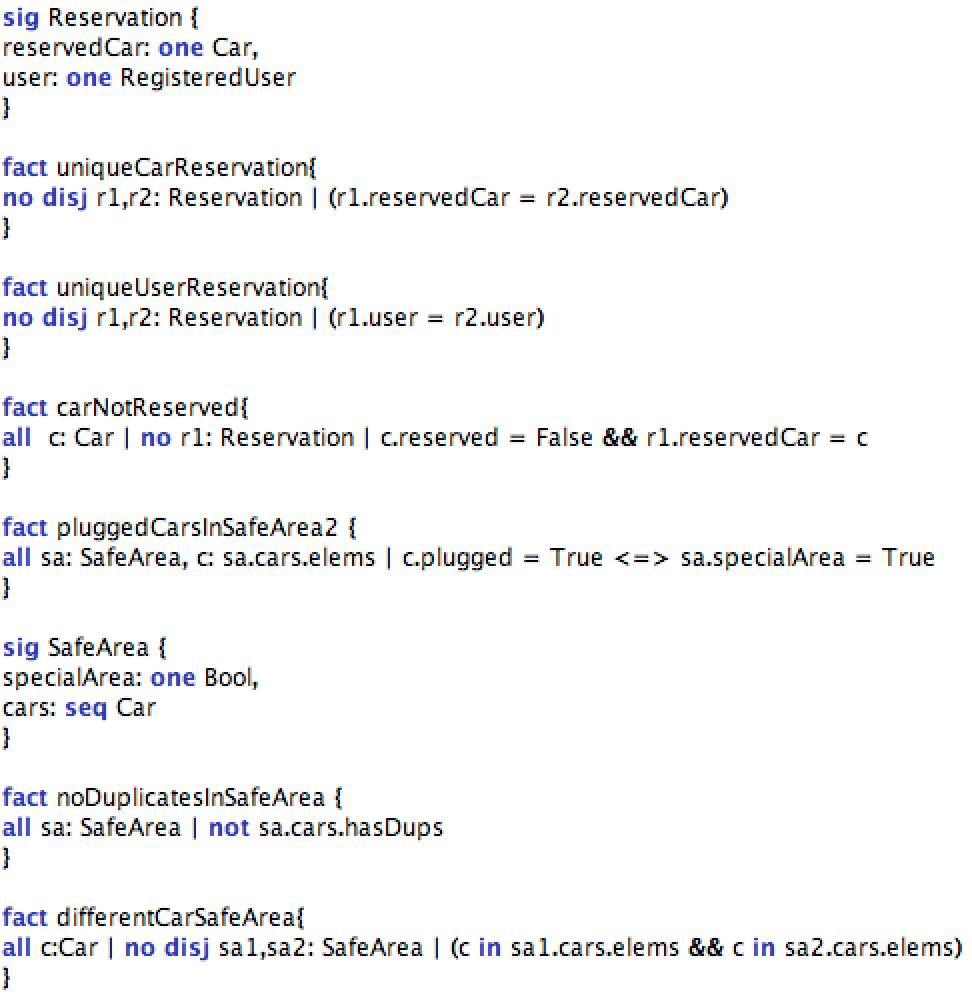
\includegraphics[width=14cm]{AlloyModel2}
\end{figure}
\begin{figure}[H]
	\centering
	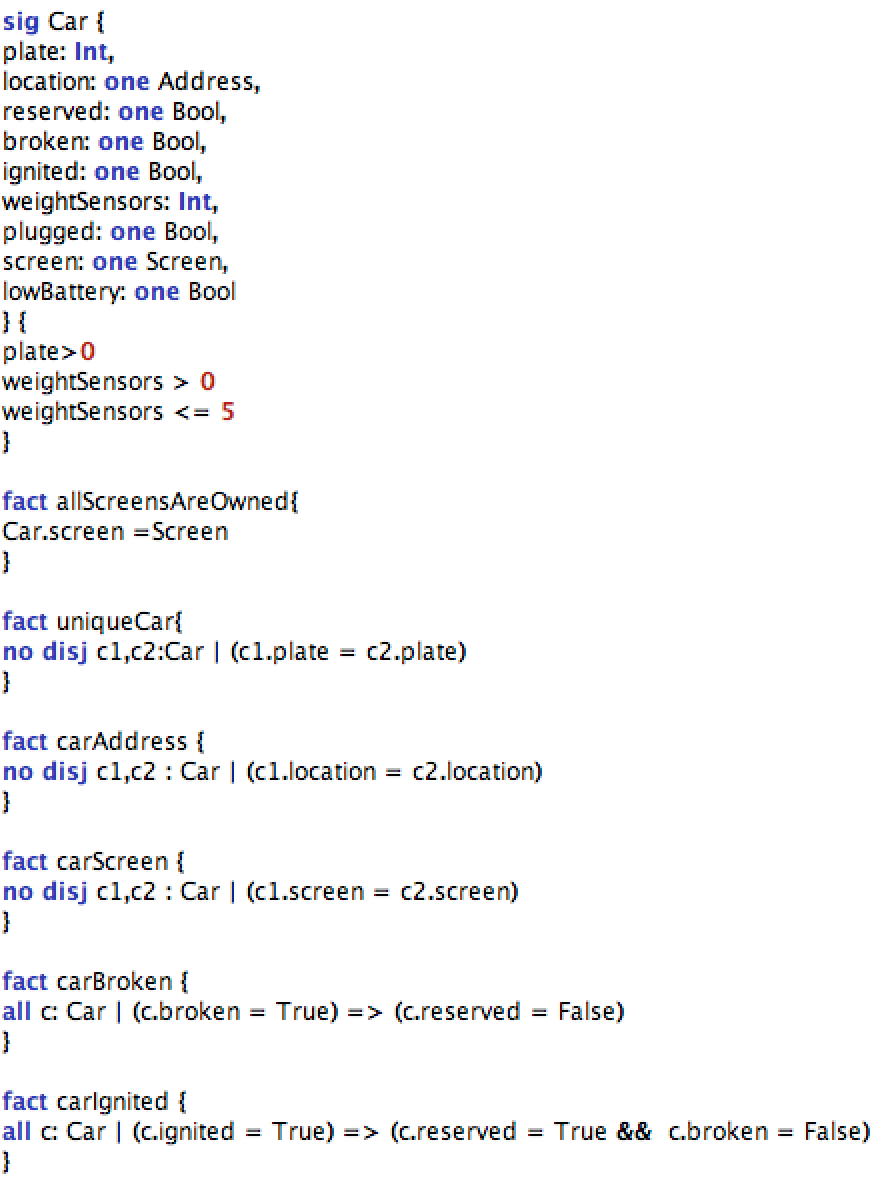
\includegraphics[width=14cm]{AlloyModel3}
\end{figure}
\begin{figure}[H]
	\centering
	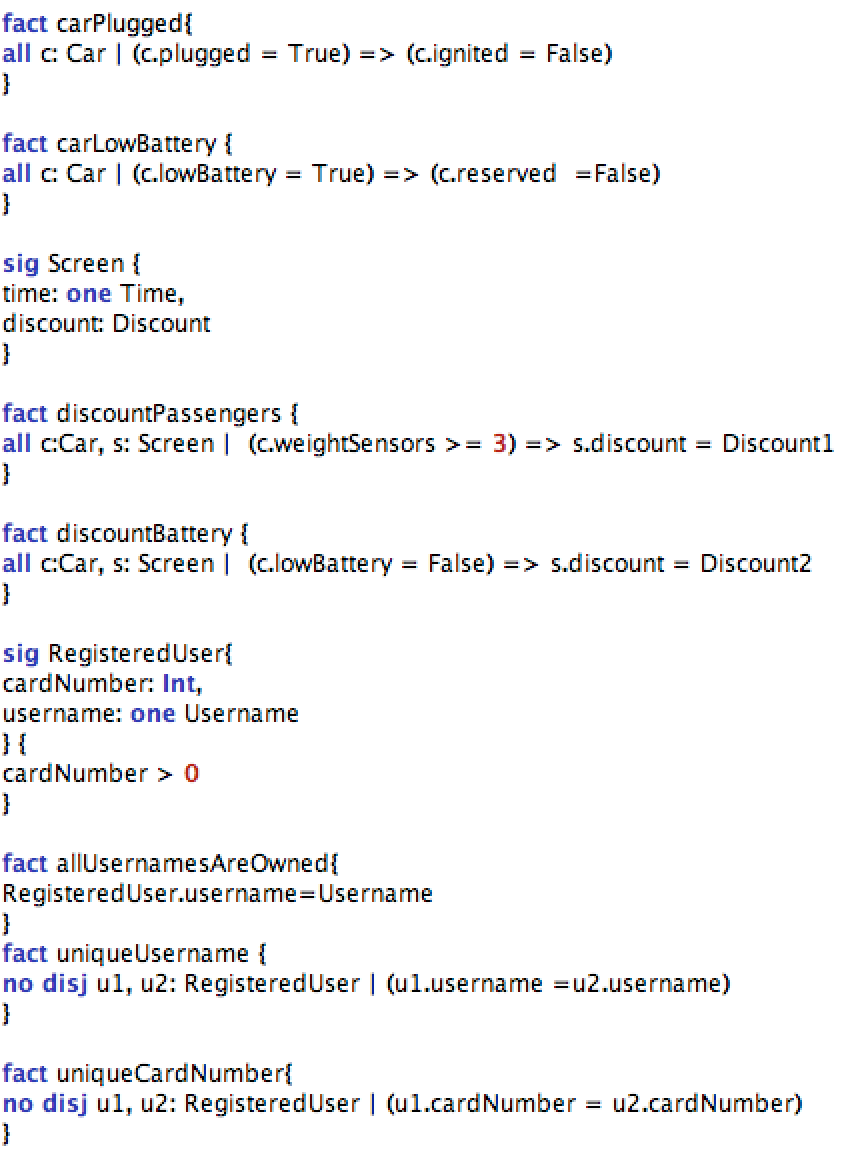
\includegraphics[width=14cm]{AlloyModel4}
\end{figure}
\begin{figure}[H]
	\centering
	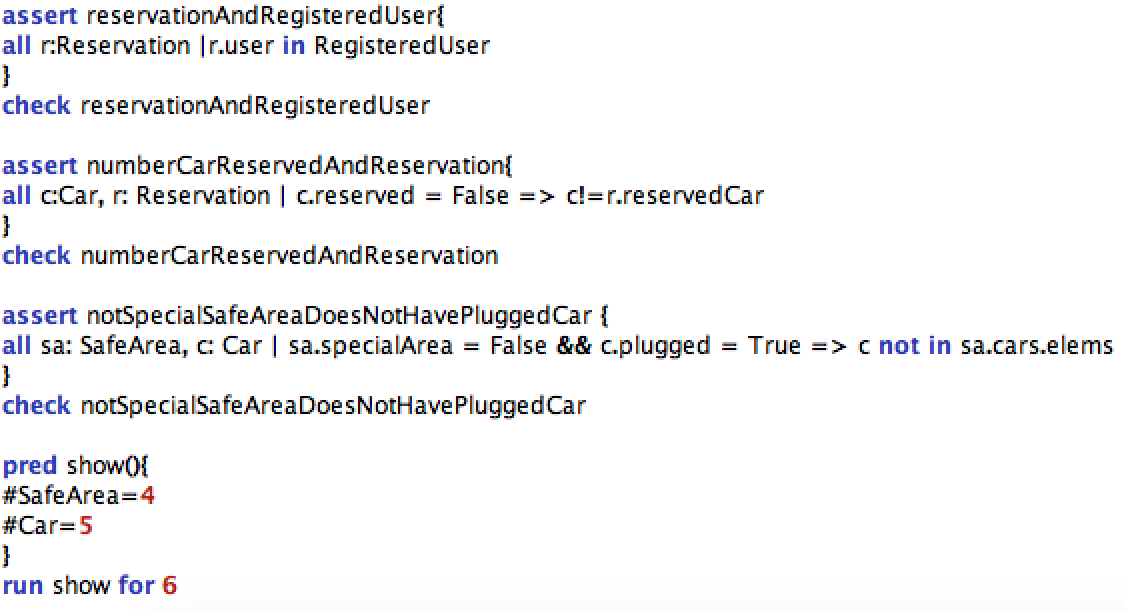
\includegraphics[width=14cm]{AlloyModel5}
\end{figure}
\subsection{Alloy result}
\begin{figure}[H]
	\centering
	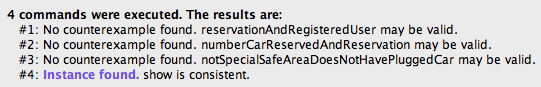
\includegraphics[width=14cm]{AlloyResult}
\end{figure}
\subsection{World generated}
\begin{figure}[H]
	\centering
	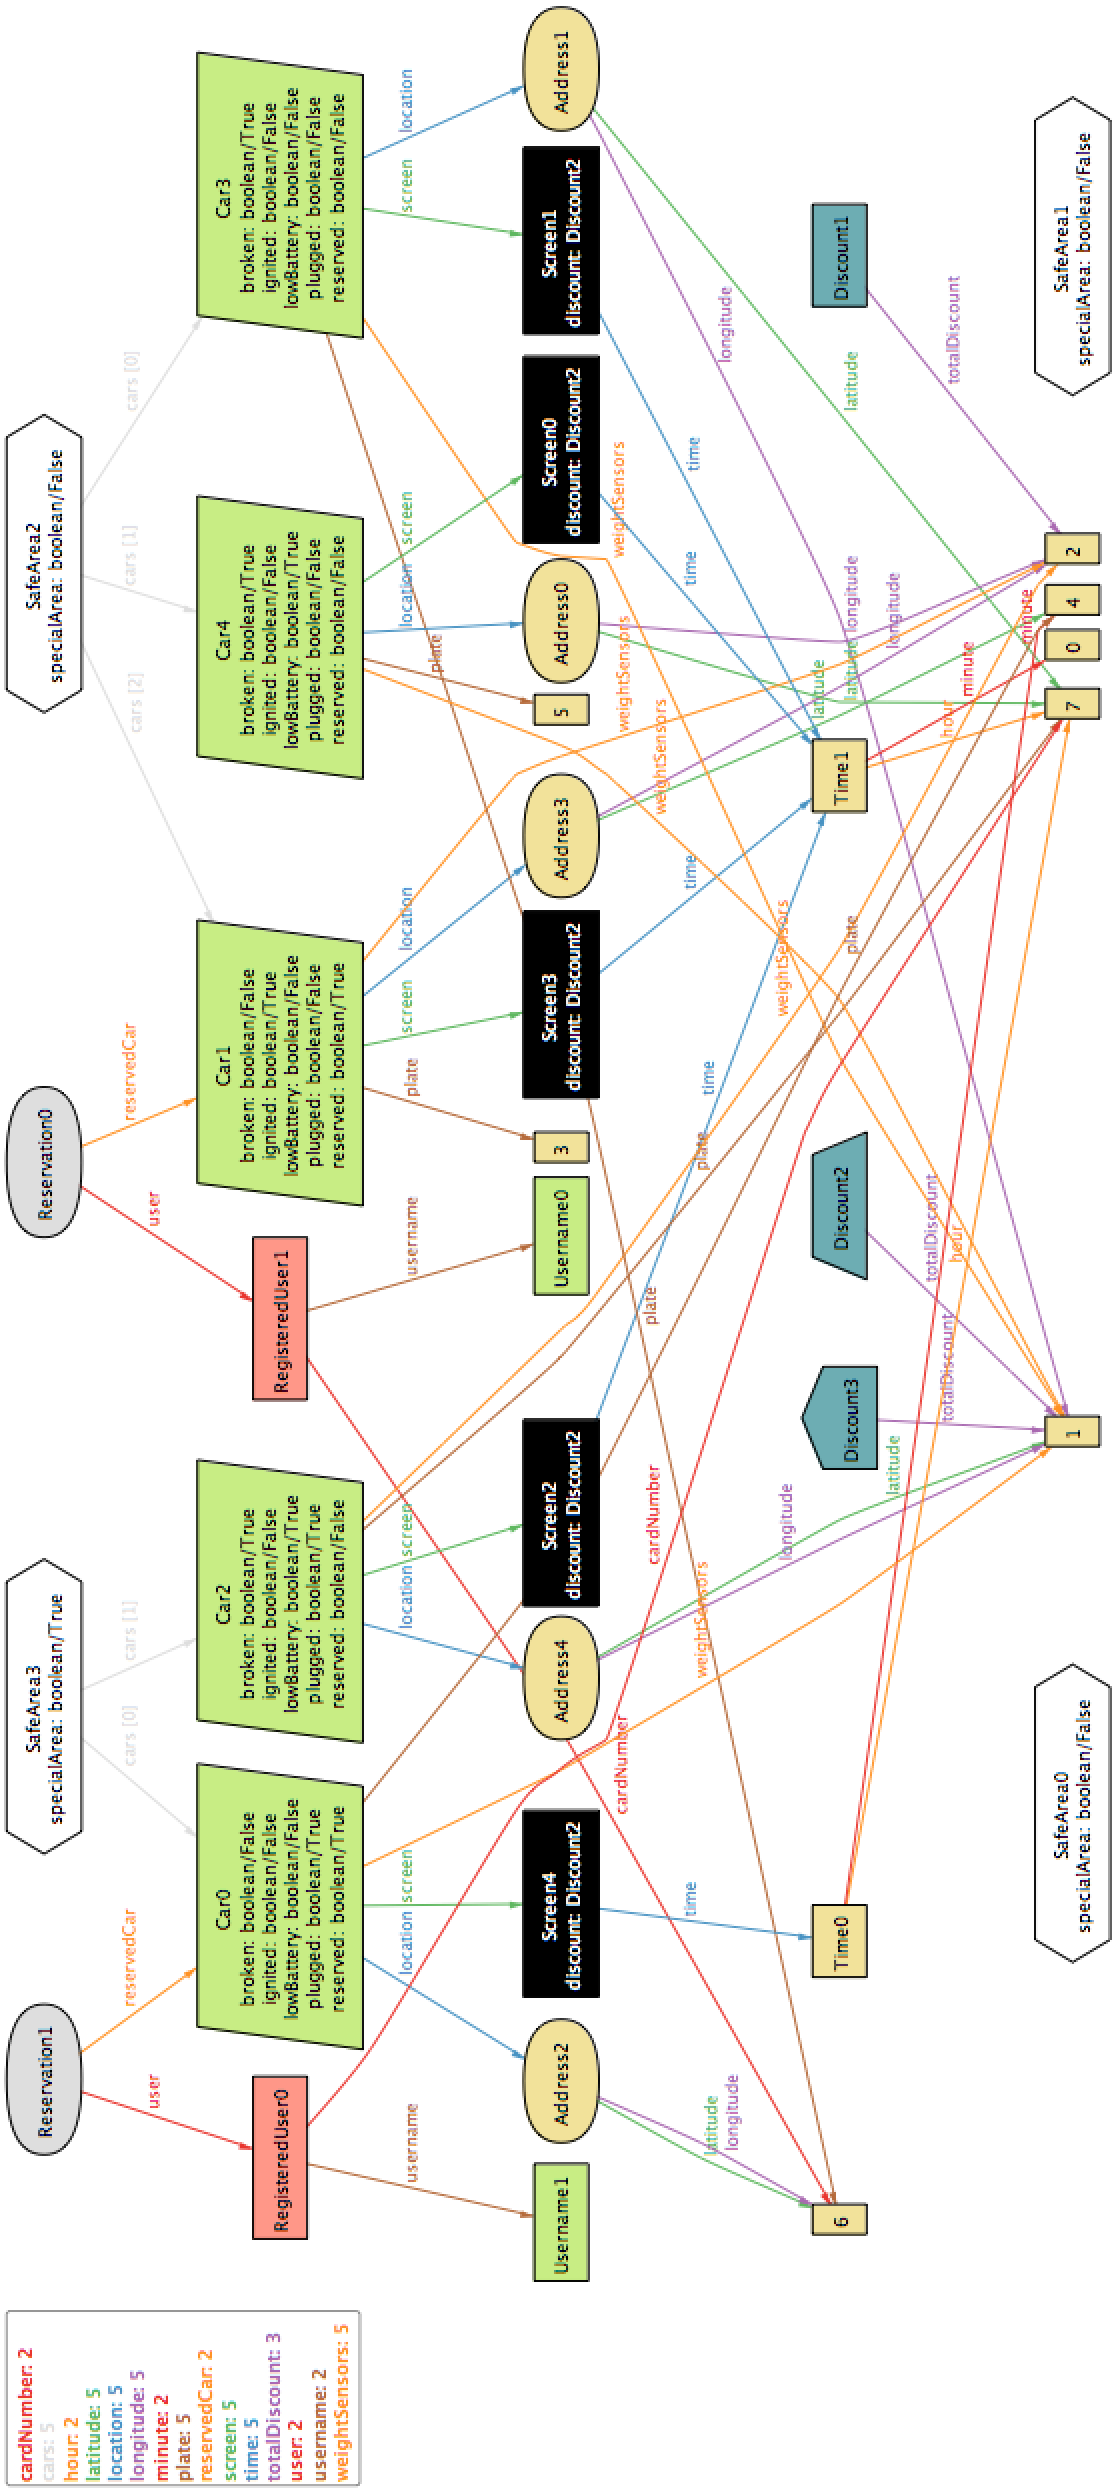
\includegraphics[height=19.5cm]{AlloyWorld}
\end{figure}